\documentclass[11pt]{article}

%% MinionPro fonts 
%\usepackage[lf]{MinionPro}
%\usepackage{MnSymbol}
\usepackage{microtype}

%% Margins
\usepackage{geometry}
\geometry{verbose,letterpaper,tmargin=1in,bmargin=1in,lmargin=1in,rmargin=1in}

%% Other packages
\usepackage{amsmath}
\usepackage{amsthm}
\usepackage[shortlabels]{enumitem}
\usepackage{titlesec}
\usepackage{soul}
\usepackage{tikz}
\usepackage{mathtools}
\usepackage{pgfplots}
\usepackage{tikz-3dplot}
\usepackage{algorithmic}
\usepackage[export]{adjustbox}
\usepackage{tcolorbox}
\usepackage{mathrsfs}

%% Paragraph style settings
\setlength{\parskip}{\medskipamount}
\setlength{\parindent}{0pt}

%% Change itemize bullets
\renewcommand{\labelitemi}{$\bullet$}
\renewcommand{\labelitemii}{$\circ$}
\renewcommand{\labelitemiii}{$\diamond$}
\renewcommand{\labelitemiv}{$\cdot$}

%% Colors
\definecolor{rred}{RGB}{204,0,0}
\definecolor{ggreen}{RGB}{0,145,0}
\definecolor{yyellow}{RGB}{255,185,0}
\definecolor{bblue}{rgb}{0.2,0.2,0.7}
\definecolor{ggray}{RGB}{190,190,190}
\definecolor{ppurple}{RGB}{160,32,240}
\definecolor{oorange}{RGB}{255,165,0}

%% Shrink section fonts
\titleformat*{\section}{\normalsize\bf}
\titleformat*{\subsection}{\normalsize\bf}
\titleformat*{\subsubsection}{\normalsize\it}

% %% Compress the spacing around section titles
\titlespacing*{\section}{0pt}{1.5ex}{0.75ex}
\titlespacing*{\subsection}{0pt}{1ex}{0.5ex}
\titlespacing*{\subsubsection}{0pt}{1ex}{0.5ex}

%% amsthm settings
\theoremstyle{definition}
\newtheorem{problem}{Problem}
\newtheorem{example}{Example}
\newtheorem*{theorem}{Theorem}
\newtheorem*{bigthm}{Big Theorem}
\newtheorem*{biggerthm}{Bigger Theorem}
\newtheorem*{bigcor1}{Big Corollary 1}
\newtheorem*{bigcor2}{Big Corollary 2}

%% tikz settings
\usetikzlibrary{calc}
\usetikzlibrary{patterns}
\usetikzlibrary{decorations}
\usepgfplotslibrary{polar}

%% algorithmic setup
\algsetup{linenodelimiter=}
\renewcommand{\algorithmiccomment}[1]{\quad// #1}
\renewcommand{\algorithmicrequire}{\emph{Input:}}
\renewcommand{\algorithmicensure}{\emph{Output:}}

%% Answer box macros
%% \answerbox{alignment}{width}{height}
\newcommand{\answerbox}[3]{%
  \fbox{%
    \begin{minipage}[#1]{#2}
      \hfill\vspace{#3}
    \end{minipage}
  }
}

%% \answerboxfull{alignment}{height}
\newcommand{\answerboxfull}[2]{%
  \answerbox{#1}{6.38in}{#2} 
}

%% \answerboxone{alignment}{height} -- for first-level bullet
\newcommand{\answerboxone}[2]{%
  \answerbox{#1}{6.0in}{#2} 
}

%% \answerboxtwo{alignment}{height} -- for second-level bullet
\newcommand{\answerboxtwo}[2]{%
  \answerbox{#1}{5.8in}{#2}
}

%% special boxes
\newcommand{\wordbox}{\answerbox{c}{1.2in}{.7cm}}
\newcommand{\catbox}{\answerbox{c}{.5in}{.7cm}}
\newcommand{\letterbox}{\answerbox{c}{.7cm}{.7cm}}

%% Miscellaneous macros
\newcommand{\tstack}[1]{\begin{multlined}[t] #1 \end{multlined}}
\newcommand{\cstack}[1]{\begin{multlined}[c] #1 \end{multlined}}
\newcommand{\ccite}[1]{\only<presentation>{{\scriptsize\color{gray} #1}}\only<article>{{\small [#1]}}}
\newcommand{\grad}{\nabla}
\newcommand{\ra}{\ensuremath{\rightarrow}~}
\newcommand{\maximize}{\text{maximize}}
\newcommand{\minimize}{\text{minimize}}
\newcommand{\subjectto}{\text{subject to}}
\newcommand{\trans}{\mathsf{T}}
\newcommand{\bb}{\mathbf{b}}
\newcommand{\bx}{\mathbf{x}}
\newcommand{\bc}{\mathbf{c}}
\newcommand{\bd}{\mathbf{d}}

%% LP format
%    \begin{align*}
%      \maximize \quad & \mathbf{c}^{\trans} \mathbf{x}\\
%      \subjectto \quad & A \mathbf{x} = \mathbf{b}\\
%                       & \mathbf{x} \ge \mathbf{0}
%    \end{align*}


%% Redefine maketitle
\makeatletter
\renewcommand{\maketitle}{
  \noindent SA405 -- AMP \hfill Rader \S 3.4 \\

  \begin{center}\Large{\textbf{\@title}}\end{center}
}
\makeatother

%% ----- Begin document ----- %%
\begin{document}
  
\title{Lesson 10.  Combinatorial Models:  Minimum Spanning Tree}

\maketitle

%%%
\section{Today...}

\begin{itemize}
	\item  Combinatorial Models
	\item  Graph Terminology
	\item  Minimum Spanning Tree (MST) Problem
	\item  MST IP Formulation
\end{itemize}

\section{Combinatorial Models}
Many optimization problems are naturally modeled by a combinatorial structure, such as a \textbf{graph}.  In this section, we will explore two famous \textbf{combinatorial optimization} problems: \emph{minimum spanning tree} and \emph{traveling salesperson}.  \emph{Shortest path} is another famous combinatorial optimization problem that we have already encountered.  SA403 Graph and Network Algorithms is all about combinatorial problems.


\begin{problem}
A local phone company is interested in laying cable from the main road (where the
Main switch is located) to a new housing subdivision, and wants to do so in the least
expensive way.  It has the option of laying cable from the road to any house, or it can 
lay cable between the houses.  Each house must be connected through some path to 
the road.  The following matrix gives the total cost of laying cable between any two
locations, where the first location is the main road.

\begin{center}
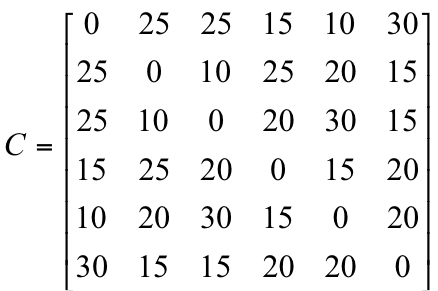
\includegraphics[width = .3\textwidth]{costs}
\end{center}

How should the phone company connect the houses to the road in order to minimize its
total cost? Brainstorm a little bit on how you might go about modeling this problem. We will come back to this later on in the lecture.
\end{problem}


%\textbf{Usually the best solution strategies for combinatorial problems are algorithms or heuristics that explicitly leverage the graphical structure of the problem.}  We will see examples of such strategies later in the course.
%
%For now, we will develop integer programs to model both classes problems.  But first we will introduce/review terminology relating to graphs.
%
%What is the difference between an \textbf{algorithm} and a \textbf{heuristic}?
%
%\answerboxfull{c}{2in}
%
%Is the simplex method an algorithm or a heuristic?
%
%\answerboxfull{c}{1in}

\newpage

\section{Graph Terminology}


Suppose $G$ is an \emph{undirected} graph. (So far we have worked with directed graphs.) Let $\mathcal{V}$ denote the set of vertices/nodes in $G$.  Let $\mathcal{E}$ denote the set of edges in $G$.  


\begin{itemize}
\item Technically, edges are \underline{unordered} pairs of vertices, since the edges in $\mathcal{E}$ are undirected. For this reason, sometimes set notation, $(i,j)$, is used to represent edges in an undirected graph.

\item When programming in Python, we have to be careful about undirected edges, because we have to use tuples (which are naturally ordered) to represent edges as keys in dictionaries. The following edge-naming convention works well:
	\begin{itemize}
		\item Use positive integers to label the vertices: $\mathcal{V} = \left\{1, 2, \dots, \left|{\mathcal{V}}\right|\right\}$.  Let $(i,j)$, \underline{where $i < j$}, represent the edge connecting vertices $i$ and $j$.  
		\item We have to keep this convention in mind as we model in Python, so we will use the same naming convention in our handwritten models.
	\end{itemize}


\item The following is some graph terminology that we will be using.
\end{itemize}

\begin{tcolorbox}
Graph $G$ is \textbf{connected} if for \emph{every} pair of vertices $a,~b \in \mathcal{V}$, there exists a \textbf{path} of edges in $G$ connecting $a$ and $b$.  
\end{tcolorbox}

\begin{tcolorbox}
A \textbf{cycle} is a sequence of connected edges that begins and ends at the same vertex.  In a cycle, no edge is repeated, and the only vertex that is visited twice is the first vertex (which is also the last).
\end{tcolorbox}

\begin{tcolorbox}
If $G$ is a connected graph that contains a \textbf{cycle}, then the removal of a single edge from the cycle does not destroy the connectivity of $G$.
\end{tcolorbox}

\begin{problem} Convince yourself of the previous fact by drawing a connected graph on 5 vertices with a single cycle.  Can you remove any edge from the graph without losing connectivity?

\answerboxone{c}{6cm}
\end{problem}


\begin{tcolorbox}
A connected graph that contains no cycles is called a \textbf{tree}.  
\end{tcolorbox}

\begin{tcolorbox}
Trees are \textbf{minimally connected}:  if we remove any edge from a tree, the resulting graph is disconnected.
\end{tcolorbox}
\begin{problem} Convince yourself of the previous fact by drawing a tree on 6 vertices.  Are there any edges you can remove from the graph without losing connectivity?

\answerboxone{c}{6cm}
\end{problem}

\newpage
\begin{tcolorbox}
A \textbf{spanning tree} of a graph $G$ is a subset of the edges of $G$ that form a 
\emph{tree that connectes every vertex in $\mathcal{V}$}.
\end{tcolorbox}


\begin{problem}
Consider any graph $G$ having 5 vertices.  

\begin{center}
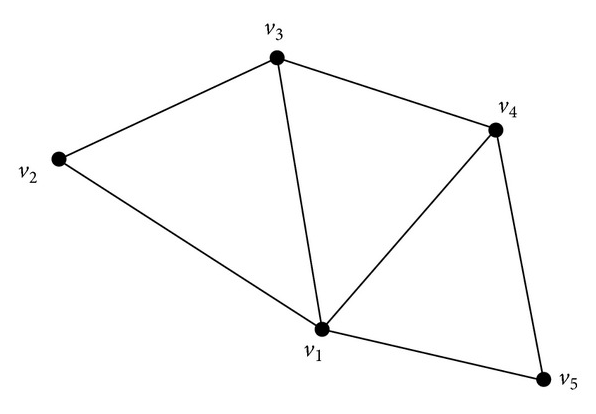
\includegraphics[width=.4\textwidth]{graph5}
\end{center}

\begin{enumerate}[(a)]
\item Draw two different spanning trees of $G$, one in each box.

\answerbox{c}{3.0in}{5cm} 
\answerbox{c}{3.0in}{5cm} 

\item How many edges does each spanning tree have?  \letterbox
\item List the elements (edges) of the spanning tree you drew on the right using the naming convention from page 1. 

	\answerboxone{c}{2cm}
\item How many edges does a spanning tree of a graph $G$ with vertex set $\mathcal{V}$ have in general?

	\answerboxone{c}{2cm}

\end{enumerate}
\end{problem}

\newpage
\section{Minimum Spanning Tree (MST) Problem}

\begin{tcolorbox}
Let $c_{ij}$ be the cost associated with every edge $(i,j) \in E$. The problem of finding the \emph{spanning tree} of graph $G$ with \emph{minimum edge cost} is known as the \textbf{minimum spanning tree problem}.
\end{tcolorbox}

\begin{itemize}
\item  Real world applications of the minimum spanning tree problem include planning road, electrical, data, phone, and water networks.  
\end{itemize}

\bigskip

\begin{problem}  Think of a military problem that could be solved by finding a minimum spanning tree.
\answerboxfull{c}{2cm}
\end{problem}

\bigskip
\begin{problem}  Solve the minimum cost spanning tree problem for the graph shown below.  (The numbers on the edges are the edge costs.)

\begin{center}
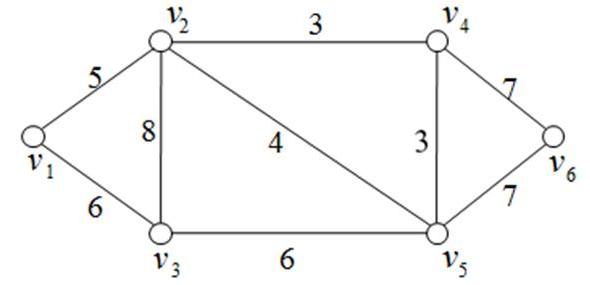
\includegraphics[width = 0.7\textwidth]{weightedgraph}
\end{center}

Minimum spanning tree $T =$   

\answerboxfull{c}{2cm}

\emph{(Provide the set of edges of the minimum cost spanning tree.  Just listing the costs of the edges is not enough information to define the solution.)}
\end{problem}


\newpage
\section{MST IP Formulation}
\emph{Note: it is more efficient to solve a min-cost spanning tree problem via an algorithm (you might learn such an algorithm in SA403).  However, as is the case for many combinatorial optimization problems, an IP formulation does not require you to write an algorithm, and can it can allow you to easily incorporate more complicated modeling elements.}

\begin{problem}
A local phone company is interested in laying cable from the main road (where the
Main switch is located) to a new housing subdivision, and wants to do so in the least
expensive way.  It has the option of laying cable from the road to any house, or it can 
lay cable between the houses.  Each house must be connected through some path to 
the road.  The following matrix gives the total cost of laying cable between any two
locations, where the first location is the main road.

\begin{center}
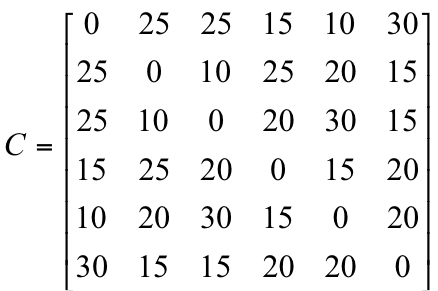
\includegraphics[width = .3\textwidth]{costs}
\end{center}

How should the phone company connect the houses to the road in order to minimize its
total cost?

\begin{enumerate}[(a)]
\item Label the rows and columns of matrix $C$ to represent nodes of the graph (using numbers). 
\item Draw the graph of the network below.  Include node labels and edge costs.

\answerboxone{c}{10cm}

\newpage
\item Define the \textbf{sets}, \textbf{variables}, and \textbf{parameters} for the problem.  Remember the edge naming convention.

\answerboxone{c}{8cm}

\item Write the objective function in concrete form, and then in abstract form.

\answerboxone{c}{8cm}

\newpage
\item Minimum spanning trees must touch every vertex.  Write a concrete constraint that ensures that vertex 1 is covered by the spanning tree returned by the solver.  Do the same for vertices 2 and 3.  Finally, write an abstract class of constraints that ensures that every vertex is covered by an edge.

\answerboxone{c}{8cm}

\item Spanning trees contain \catbox edges.  Write a concrete constraint that ensures that the solution returned by the solver has exactly \letterbox edges.  Convert this constraint to abstract form.

\answerboxone{c}{8cm}

\newpage
\item Do we have all of the constraints that we need?  Can you think of a subgraph of the graph $G$ associated with this problem that contains the correct number of edges and touches every vertex, but is not connected?  Sketch this graph below.

\answerboxone{c}{6cm}

\item Write a concrete constraint that prevents the graph that you sketched above.  Then write a set of abstract constraints that prevents ANY graphs of this kind from being returned by the solver.  (There is one such constraint for every subset $S$ of vertices of $G$, such that $|S| \geq 3$.)

\answerboxone{c}{8cm}



\end{enumerate}

\end{problem}

\begin{tcolorbox}
The constraints above are called \textbf{cycle-elimination} constraints.  In real-life applications, there are usually way too many possible ``cycle-elimination'' constraints to include them all in a model.  In practice, these constraints may be added iteratively to eliminate cycles in a solution returned by the solver. 
\end{tcolorbox}


\end{document}
